\documentclass{article} % For LaTeX2e
\usepackage{nips14submit_e,times}
\usepackage{amsmath}
\usepackage{amsthm}
\usepackage{amssymb}
\usepackage{mathtools}
\usepackage{hyperref}
\usepackage{url}
\usepackage{algorithm}
\usepackage[noend]{algpseudocode}
%\documentstyle[nips14submit_09,times,art10]{article} % For LaTeX 2.09

\usepackage{graphicx}
\usepackage{caption}
\usepackage{subcaption}

\def\eQb#1\eQe{\begin{eqnarray*}#1\end{eqnarray*}}
\def\eQnb#1\eQne{\begin{eqnarray}#1\end{eqnarray}}
\providecommand{\e}[1]{\ensuremath{\times 10^{#1}}}
\providecommand{\pb}[0]{\pagebreak}

\newcommand{\E}{\mathrm{E}}
\newcommand{\Var}{\mathrm{Var}}
\newcommand{\Cov}{\mathrm{Cov}}

\def\Qb#1\Qe{\begin{question}#1\end{question}}
\def\Sb#1\Se{\begin{solution}#1\end{solution}}

\newenvironment{claim}[1]{\par\noindent\underline{Claim:}\space#1}{}
\newtheoremstyle{quest}{\topsep}{\topsep}{}{}{\bfseries}{}{ }{\thmname{#1}\thmnote{ #3}.}
\theoremstyle{quest}
\newtheorem*{definition}{Definition}
\newtheorem*{theorem}{Theorem}
\newtheorem*{lemma}{Lemma}
\newtheorem*{question}{Question}
\newtheorem*{preposition}{Preposition}
\newtheorem*{exercise}{Exercise}
\newtheorem*{challengeproblem}{Challenge Problem}
\newtheorem*{solution}{Solution}
\newtheorem*{remark}{Remark}
\usepackage{verbatimbox}
\usepackage{listings}
\title{Human Genetics: \\
Problem Set XI}


\author{
Youngduck Choi \\
New York University\\
\texttt{yc1104@nyu.edu} \\
}


% The \author macro works with any number of authors. There are two commands
% used to separate the names and addresses of multiple authors: \And and \AND.
%
% Using \And between authors leaves it to \LaTeX{} to determine where to break
% the lines. Using \AND forces a linebreak at that point. So, if \LaTeX{}
% puts 3 of 4 authors names on the first line, and the last on the second
% line, try using \AND instead of \And before the third author name.

\newcommand{\fix}{\marginpar{FIX}}
\newcommand{\new}{\marginpar{NEW}}

\nipsfinalcopy % Uncomment for camera-ready version

\begin{document}


\maketitle

\begin{abstract}
This work contains the solutions to the problem set XI
of Human Genetics 2015 course at New York University.
\end{abstract}

\bigskip

\begin{question}[1]
\hfill
\begin{figure}[h!]
  \centering
    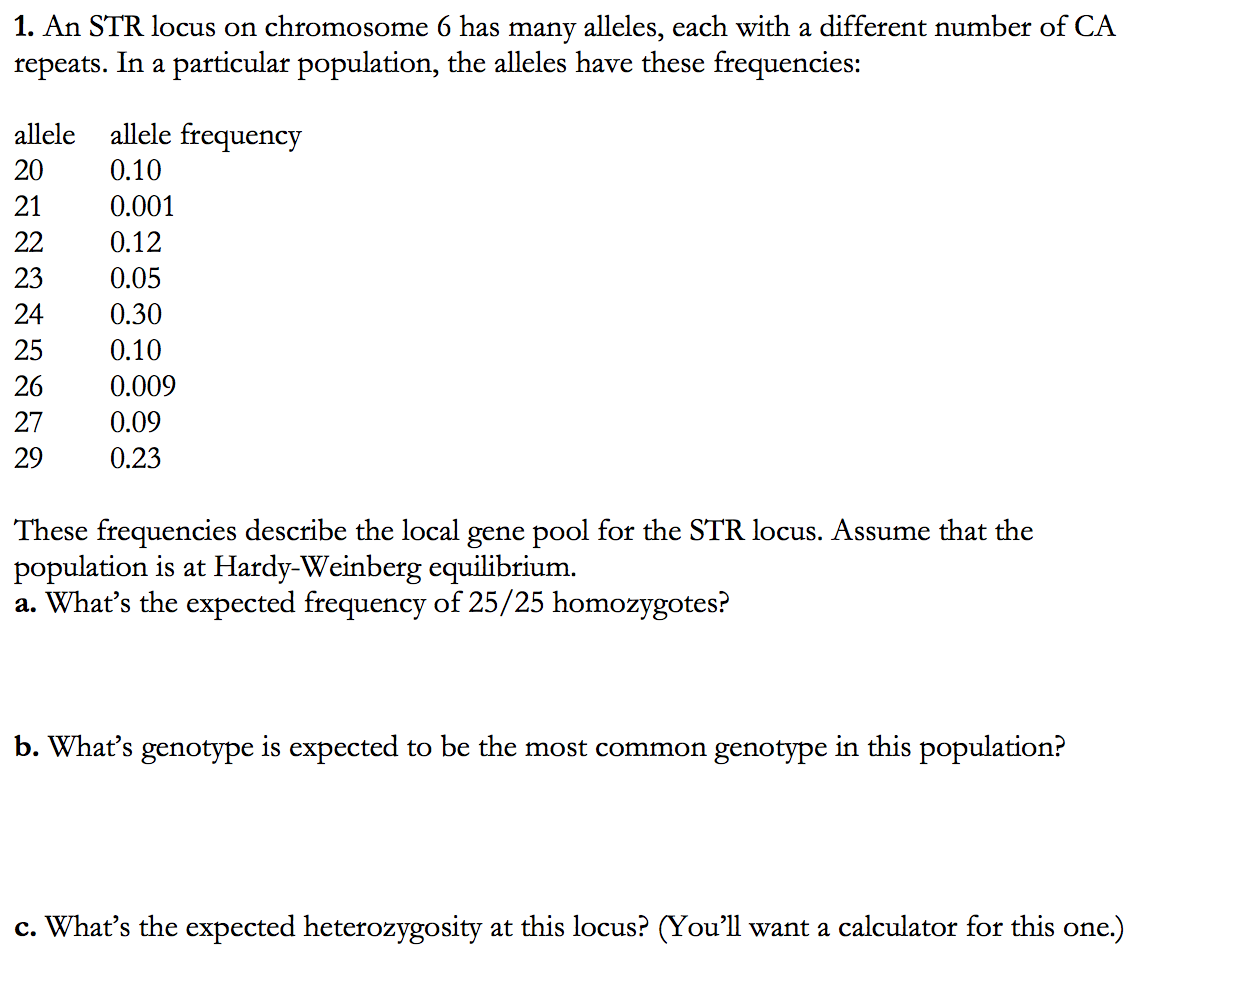
\includegraphics[width=1\textwidth]{genetics-9-1.png}
\end{figure}
\end{question}
\newpage

\begin{solution}
\textbf{(a)} The expected frequency of $25/25$ homozygotes is $0.1^2 
= 0.01$.

\smallskip

\textbf{(b)} The most common genotype in this population will be
$24 \// 29$ heterozygote with $2\cdot 0.30 \cdot 0.23$ chance. 

\smallskip

\textbf{(c)} The expected heterozygosity at this locus, can be
computed by $1 - \sum_{locus} p_{locus}^2$, where $p_{locus}$
is the allele frequency at a particular locus. Carrying out the
calculations, we obtain that the expected heterozygosity is approximately  
$0.812$

\hfill $\qed$

\end{solution}

\newpage

\begin{question}[2]
\hfill
\begin{figure}[h!]
  \centering
    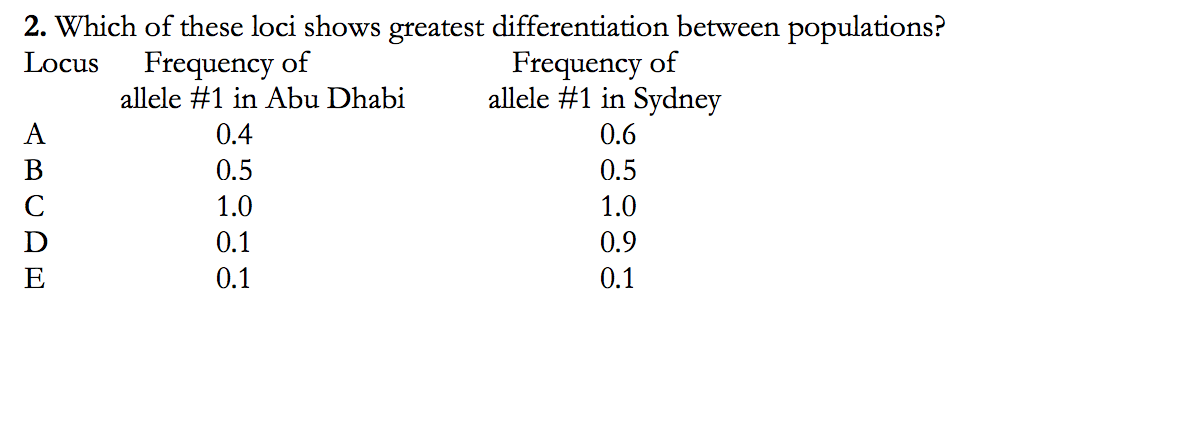
\includegraphics[width=1\textwidth]{genetics-9-2.png}
\end{figure}
\end{question}
\begin{solution}
By referring to the differentiation map, we see that the $(0.1,0.9)$ 
pair of allele frequency results in the highest differentiation. Hence,
the $D$ locus shows the greatest differentiation between populations.
\hfill $\qed$ 
\end{solution}

\newpage

\begin{question}[3]
\hfill
\begin{figure}[h!]
  \centering
    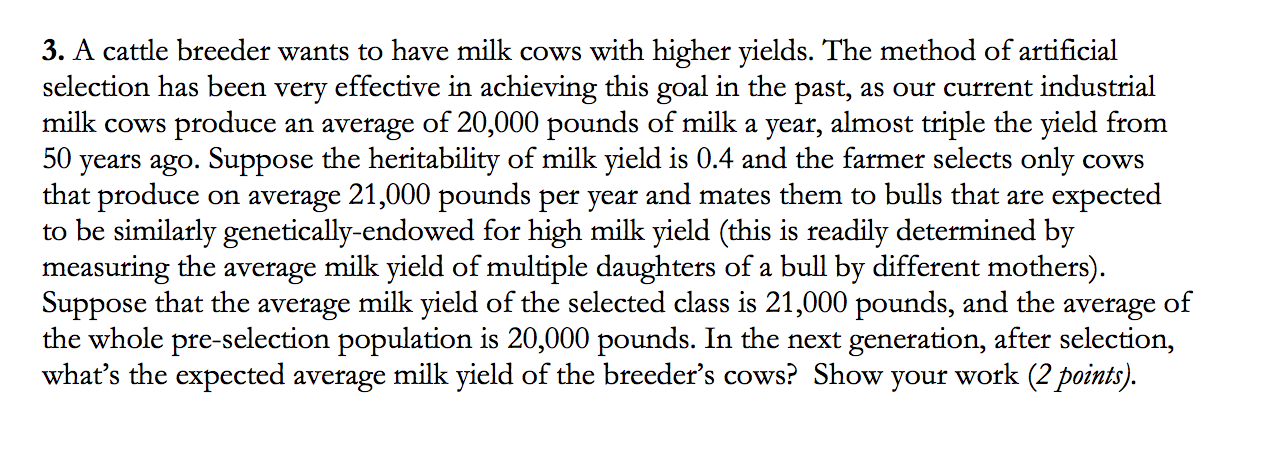
\includegraphics[width=1\textwidth]{genetics-9-3.png}
\end{figure}
\end{question}
\begin{solution}
Observe that the selection differential is $21000 - 20000 = 1000$ and
heritability is $0.4$. Hence, the Breeder's equation gives that
the response to selection is $400$. Hence, the expected
average milk yield of the breeder's cows is $21000 - 400 = 20600$. 
\hfill $\qed$
\end{solution}

\newpage 

\begin{question}[4]
\hfill
\begin{figure}[h!]
  \centering
    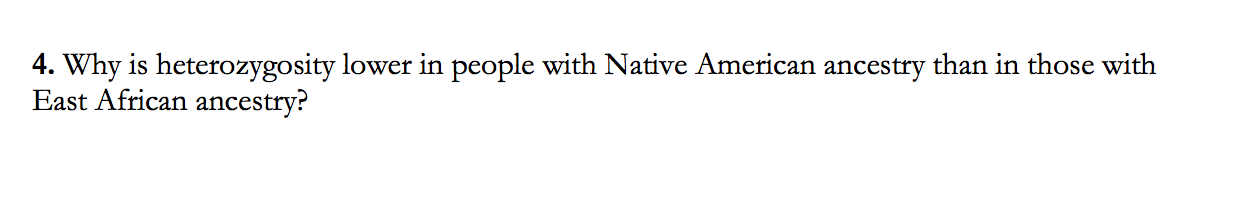
\includegraphics[width=1\textwidth]{genetics-9-4.png}
\end{figure}
\end{question}
\begin{solution}
The founders effect tells us that the expected heterozygosity 
decreases as the population is located further away from East
Africa. Therefore, people with the Native American ancestry 
has lower heterozygosity than those with East African ancestry. 
\hfill $\qed$ 
\end{solution}

\newpage

\begin{question}[5]
\hfill
\begin{figure}[h!]
  \centering
    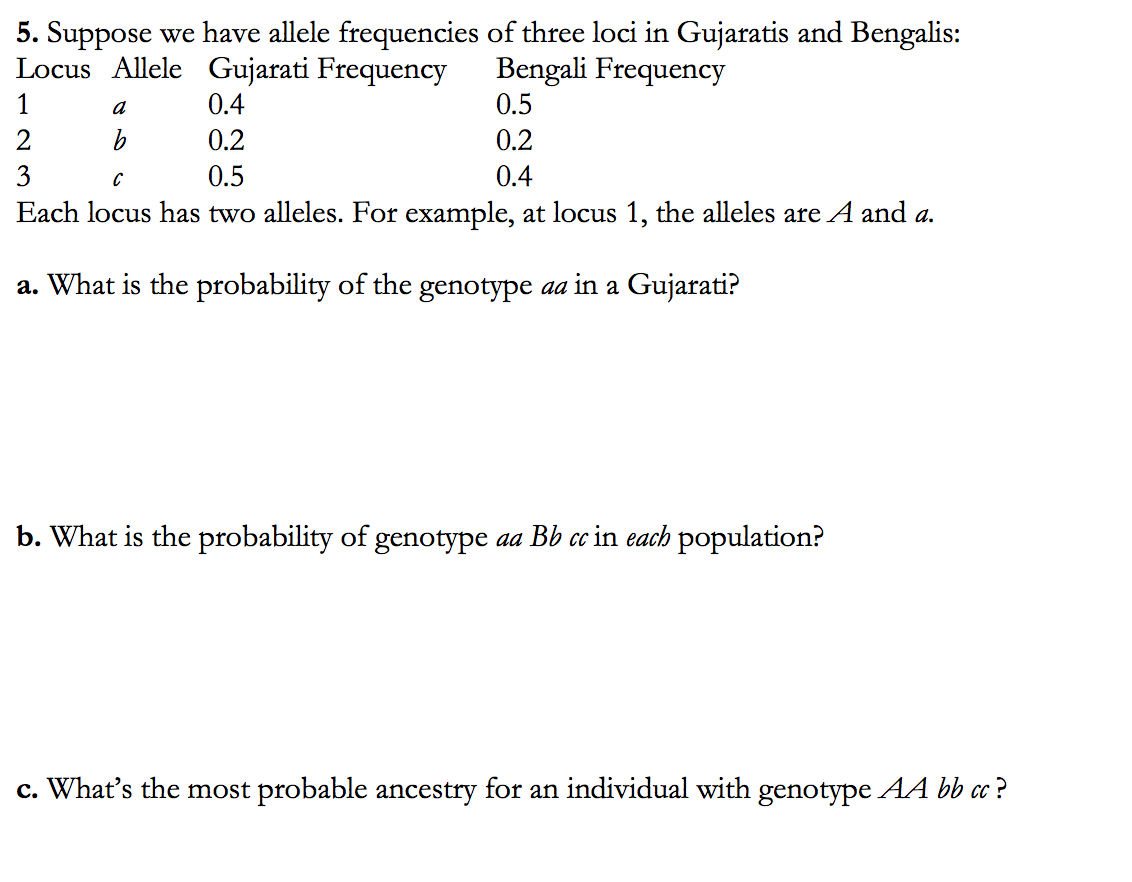
\includegraphics[width=1\textwidth]{genetics-9-5.png}
\end{figure}
\end{question}
\begin{solution}
\textbf{(a)} The probability of the genotype $aa$ in Gujarati is
$0.4^2 = 0.16$.

\smallskip

\textbf{(b)} The probability of the genotype of aa Bb cc for Gujarati is
$0.4^2 \cdot 2\cdot 0.8 \cdot 0.2 \cdot 0.5^2 \approx 0.128$.
The probability of the genotype of aa Bb cc for Bengali is
$0.5^2 \cdot 2 \cdot 0.2 \cdot 0.8 \cdot 0.4^2 \approx 0.128 $, which equals
that of Gujarati. 
 
\smallskip

\textbf{(c)} The probability of the genotype of AA bb cc for
Gujarati is $0.6^2 \cdot 0.2^2 \cdot 0.5^2 \approx 0.0023$. The probability
of the genotype of AA bb cc for Bengali is $0.5^2 \cdot 0.2^2 \cdot 0.4^2
= 0.0016$. Hence, the most probable ancestry for an individual with
genotype AA bb cc is Gujarati. 

\hfill $\qed$

\end{solution} 

\end{document}

